
\documentclass[10pt,letterpaper]{article}
\usepackage[top=0.85in,left=0.85in,footskip=0.75in]{geometry}
% amsmath and amssymb packages, useful for mathematical formulas and symbols
\usepackage{amsmath,amssymb}
% Use adjustwidth environment to exceed column width (see example table in text)
\usepackage{changepage}
% Use Unicode characters when possible
\usepackage[utf8x]{inputenc}
% textcomp package and marvosym package for additional characters
\usepackage{textcomp,marvosym}
% cite package, to clean up citations in the main text. Do not remove.
\usepackage{cite}
\usepackage{url}
% Use nameref to cite supporting information files (see Supporting Information section for more info)
%\usepackage{nameref,hyperref}
% line numbers
%\usepackage[right]{lineno}

%\usepackage{natbib}
\usepackage{graphicx}
\usepackage{float}

% color can be used to apply background shading to table cells only
\usepackage[table]{xcolor}

% array package and thick rules for tables
\usepackage{array}
\usepackage{dsfont}

\usepackage{todonotes}
\usepackage{comment}

% referencing supplement-material
\usepackage{xr}
\externaldocument{./supplement}
%\usepackage{cleveref}



%% END MACROS SECTION

\title{Triqler for Protein Summarization of Data from Data Independent Aquisition Mass Spectrometry}
\author{Patrick Truong \and Matthew The \and Lukas K\"{a}ll}


\begin{document}
%\linenumbers
\maketitle

%Here I want to reference a figure that is in my supplementary content \cref{supp-fig:model_selection_criteria}.

%Here is a ref to the supplement, we have a Supplementary Figure \ref{fig:diff_vs_hela_find_a_better_label}.

\begin{abstract}

A frequent goal, or subgoal, when processing data from a quantitative shotgun proteomics experiment is a list of proteins that are differentially abundant under the examined experimental conditions. Unfortunately, obtaining such a list is a challenging process, as the mass spectrometer analyses the proteolytic peptides of a protein rather than the proteins themselves. We have previously designed a Bayesian hierarchical probabilistic model, Triqler, for combining peptide identification and quantification errors into probabilities of proteins being differentially abundant. 

Here we show that Triqler is compatible with data-independent acquisition data after applying minor alterations for the missing value distribution. Furthermore, we find that it has better performance than other protein summarization tools when compared to a set of state-of-the-art DIA processing methods.
\end{abstract}
  
\listoftodos
\section*{Introduction}

Mass spectrometry (MS)-based proteomics enables efficient detection of proteins in complex mixtures. There are several different techniques to make the technology quantitative \cite{bantscheff2007quantitative,kall2011computational}. Out of these, label-free quantification (LFQ) \cite{bondarenko2002identification} has the advantage that it can handle large sample sizes in a straightforward manner. For data from LFQ experiments, just as in other quantification schemes, there exists a plethora of processing options, all containing several processing steps, each subject to their different error sources, all affecting the result of the processing.


We have previously designed a hierarchical Bayesian model, Triqler, able to control for errors from both the identification and quantification process in LFQ experiments\cite{the2019integrated}. By integrating the error probabilities from identification and quantification, one can obtain better accuracy in calling differentially abundant proteins. Triqler does so by assuming that peptide abundances follow a probability distribution. This abundance distribution is initiated according to a prior distribution, but updated based on each samples registered peptide ambundance values. This results in peptide abundance distributions that are integrated into protein abundance and subsequently fold change distributions. In the processing Triqler weights in information on differences of peptide abundances within sample groups and search engine identification error probabilities. Data that indicate uncertanty results in wider abundance distributions, while certainty result in tighter abundance distributions. Triqler also integrates the resulting fold change distributions to dereive a posterior probabilities for each protein having an actual fold change larger than a preset treshold value. These posterior probabilities are also averaged into $q$~values \cite{the2019integrated}.

Triqler was originally designed for handling LFQ data from Data-dependent acquisition (DDA). However, in principle, once once peptide abundances and identities are estimated, there are only small differences between data from DDA and Data-independent acquisition (DIA) mass spectrometry \cite{venable2004automated}. Here, we set out to investigate Triqler's ability to summarize protein concentrations from peptide abundances derived from DIA data. We used the LFQBench from Navarro et al. \cite{navarro2016multicenter} for the evaluation. In the original benchmark, Navarro et al. included a comparison of different protein summarization strategies and found that the so-called Top3 method generally resulted in lower variance and better quantification accuracy than the built-in methods from OpenSwath, SWATH2.0, Skyline, Spectronaut, and DIA-Umpire\cite{navarro2016multicenter}. However, there are reasons to believe that more sophisticated methods would yield better protein quantification than the Top3-method. Simple summarization methods based on mean and median peptide intensity have been shown to produce unreliable protein abundance estimates \cite{goeminne2015summarization}, and more advanced summarization strategies for LFQ data have been proposed in the literature \cite{silva2006absolute,cox2014accurate}. Summarization techniques such as PQPQ~\cite{forshed2011enhanced}, MSstats~\cite{choi2014msstats}, Diffacto~\cite{zhang2017covariation}, MSqRob2~\cite{sticker2020robust} and Triqler~\cite{the2019integrated} have all been shown to outperform Top3 and there are no theoretical reasons why the stated methods would not perform well for DIA data. Hence, we found it apt to benchmark Triqler against a set of state-of-the-art protein summarization methods using peptide quantities from the LFQBench DIA data set.
\todo{Add description of ``biological'' study. Possibly also to the abstract.} 
 
\section*{Materials and methods}


%\subsection*{Data description}
\subsubsection*{LFQBench mass spectrometry data}


We downloaded the LFQBench dataset~\cite{navarro2016multicenter} from PRIDE (PXD002952). Here we used the TripleTOF6600 section of the study, which was harvested with a setup of 32 fixed windows MS2-windows. We also restricted ourselves to the low ratio difference samples, referred to as the HYE124 hybrid proteome samples in the original study. These consist of triplicates of Sample A composed of tryptically digested proteins from 65\% w/w HeLa, 30\% w/w yeast, and 5\% w/w \textit{E. coli} cells, and triplicates of Sample B, composed of 65\% w/w, 15\% w/w yeast, and 20\% w/w \textit{E. coli} proteins. Samples from HYE110 and the TripleTOF5600 section of PXD002952 were omitted in this study. Further details about mass spectrometric instrumentation and data acquisition are available in Navarro et al.~\cite{navarro2016multicenter}. The \verb|.wiff| files were converted to \verb|.mzML| files in a centroided format using msconvert (using Windows OS msconvert version 3.0) with peakPicking filter msLevel=1-). 

\subsubsection*{LFQBench sequence database}

Uniprot FASTA files with one protein sequence per gene were downloaded for each species (UP000005640, UP000000625, and UP000002311, acquired on 2021-06-16). The unfiltered FASTA files contained 20 590 human proteins, 6 046 yeast proteins, and 4 373 \textit{E. coli} proteins. To reduce the effect of the different protein inference strategies for the tested protein summarization tools, a modified FASTA file, without shared peptides, was used for database search. The filter removed protein sequences with shared peptides so that the final database did not contain any two proteins sharing tryptic peptides longer than 7 amino acids. After filtering the FASTA file contained 20 302 proteins (288 human proteins fewer proteins than an unfiltered database), 5 848 yeast proteins (198 yeast proteins fewer proteins than an unfiltered database), and 4 306 \textit{E. Coli} proteins (67 \textit{E. Coli} proteins than an unfiltered database). Replacing the I/L amino acids to handle the mass equivalence did not result in any considerable differences (See Supplementary Table \ref{table:proteins_in_database}). We also added pseudo-reverse sequences to the database as decoys for target-decoy analysis using OpenSwathDecoyGenerator. 

\subsubsection*{Cancer proteomics study}
TWe downloaded DIA data from  frozen lung squamous cell carcinomas and four adjacent tissues, from the proteomeexchange project PXD004684.
\todo{description of sources of data here.}

\subsection*{General workflow}

We used two separate strategies to generate peptide abundances from the DIA runs. First, we used a spectral library consisting of selected spectra from separate DDA runs, we refer to this workflow as ID hereon, and secondly, we searched pseudo-spectra generated directly from the DIA data, we will refer to this workflow as PS from hereon. The workflows are shown in Figure \ref{fig:flowchart}. We will describe the parameter choices of both these two methods below.

\begin{figure}[htp]
    \centering
    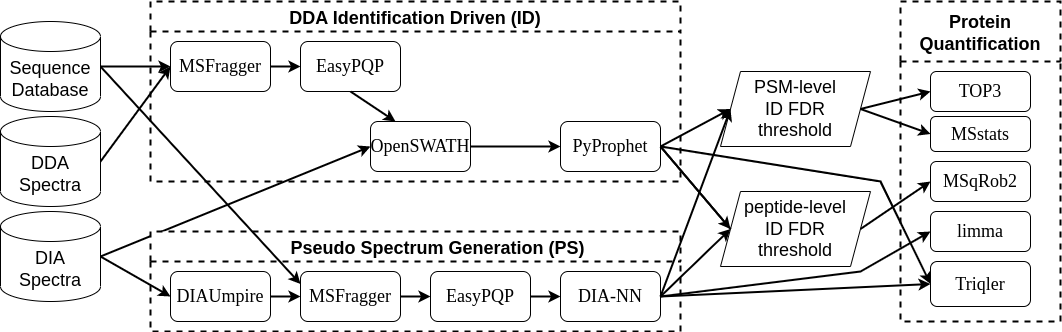
\includegraphics[width=1.0\linewidth]{./img/methods.png} 
    \caption{{\bf The DDA identification-driven matching (ID) and pseudo-spectrum workflow pipelines (PS).} In the pipelines DIA-Umpire(SE), MSFragger and EasyPQP are run from Fragpipe (\protect\url{https://fragpipe.nesvilab.org/}). A 1\% PSM-level identification threshold was applied to Top3 and MSstats, a 1\% peptide-level threshold to MSqRob2, while all the identifications were provided unfiltered to Triqler. \label{fig:flowchart}}  
\end{figure}



\subsubsection*{DDA identification-driven (ID) spectral library}

For the ID workflow, we searched the LFQBench provided DDA runs with MSFragger\cite{kong2017msfragger} with default settings (Precursor mass tolerance of [-20, 20] ppm, fragment tolerance of 20 ppm, Calibration and Optimization: ``Max calibration, parameter optimization'', isotope error: 0/1, Data type: DDA, Load rules: stricttrypsin, Cut after: KR, Cleavages: ENZYMATIC, Missed cleavages: 2, Clip N-term M: True, Peptide length of [7, 50], Peptide mass range of [500, 5000], Split database: 1, and allowing for oxidation on methionine and protein N-terminus modifier as variable modifications), and a spectral library was constructed with EasyPQP \cite{easypqp} with the default setting (RT Calibration: ``Automatic selection of a run as reference RT'', RT Lowess Fraction: 0.1, UniMod annotation tol(Da), Fragment annotation tol(ppm): 15, and the default PSM-level threshold of 0.01, peptide-level false discovery rate (FDR) of 0.01, and protein-level FDR of 0.01). No transition refinement was used. OpenSwatchDecoyGenerator was used to generate decoys for the spectral library with a pseudo-reverse method. The DIA data was searched with the spectral library through OpenSwath Workflow, and the \texttt{m\_score} was computed using PyProphet\cite{teleman2015diana}. The \texttt{m\_score} cut-off for a user-specified peptide identification false-discovery rate was computed with SWATH2STATS \cite{blattmann2016swath2stats}. This process resulted in a set of detected peptides together with their assessed peptide identification accuracies and abundance estimates (Supplementary Table \ref{fig:osw_peptide_and_protein_id} shows the number of identified peptides and proteins).


\subsubsection*{Pseudo-spectra generation (PS) spectral library}

For the PS workflow, we also used the FragPipe software, employing DIA-Umpire to extract pseudo-spectra from the DIA data. The DIA-Umpire parameters was set to default values (MS1 PPM: 10, MS2 PPM: 20, Max Missed Scans: 1, Mass Defect Filter: True, RP max: 25, RF max: 500, Corr Threshold: 0, Delta Apex: 0.2, RT Overlap 0.3, Mass Defect Offset 0.1, Isotope Pattern: 0.3, MS1 SN: 1.1, MS2 SN: 1.1, Adjust Fragment Intensity: True). The pseudo-spectra were subsequently searched using MSFragger with default settings (Precursor mass tolerance of [-20, 20] ppms, fragment tolerance of 20 ppms, Calibration and Optimization: ``Max calibration, parameter optimization'', isotope error: 0/1, Data type: DDA, Load rules: stricttrypsin, Cut after: KR, Cleavages: ENZYMATIC, Missed cleavages: 2, Clip N-term M: True, Peptide length of [7, 50], Peptide mass range of [500, 5000], Split database: 1, and allowing for oxidation on methionine and protein N-terminus modifier as variable modifications). A spectral library was built from the resulting PSMs using easyPQP with default setting (RT Calibration: ``Automatic selection of a run as reference RT'', RT Lowess Fraction: 0.1, UniMod annotation tol(Da), Fragment annotation tol(ppm): 15, and the default PSM-level threshold of 0.01, peptide-level FDR of 0.01, and protein-level FDR of 0.01). DIA-NN (version 1.7.12) was used for peptide quantifications with settings specified in \url{https://fragpipe.nesvilab.org/docs/tutorial_DIA.html#quantify-with-dia-nn} (Protein inference: ``Off'', Quantification strategy: ``Robust LC (High accuracy)'', Precursor FDR (\%): 1.0, Protease: ``Trypsin/P'', Missed cleavages: 1, Maximum number of variable modifications: 0, N-term M excision: True, C carbamidomethylation: True, Peptide length: [7, 30], Precursor m/z range: [300, 1800], Fragment ion m/z range: [200, 1800], Mass accuracy: 0.0, MS1 accuracy: 0.0, Scan window: 0, Use isotopologues: True, Remove likely interferences: True, Neural network classifier: ``Single-pass mode'', Protein inference: Genes, Cross-run normalization: ``RT-dependent'', Library generation: ``Smart profiling''). To compute false discovery rates, DIA-NN uses a built-in custom implementation of the mProphet algorithm\cite{reiter2011mprophet, demichev2020dia} (Supplementary Table \ref{fig:diann_peptide_and_protein_id} shows the number of identified peptides and proteins). 


\subsection*{Protein summarization}

The peptide quantities were summarized to proteins using the average of the three most intense peptides (We call it Top3), MSstats, MSqRob2, and Triqler. This is done for both the ID and PS pipelines. 

\subsubsection*{Top3}

We implemented a short script that takes the average of the 3 most abundant PSMs for each protein and sample. In samples only having two PSMs these were also included, still represented by their average. Proteins with one or zero PSMs per sample were excluded. PSMs were filtered at a 1\% PSM-level FDR before performing the Top3 protein summarization. 

\subsubsection*{MSstats}

We installed MSstats version 3.18.5 using R/Bioconductor (available at \url{https://www.bioconductor.org/packages/release/bioc/html/MSstats.html}). MSstats use feature-level data, allowing for multiple PSM hits per peptide identification. We use the disaggregate function to disaggregate the PSMs to fragment-level data. We filtered so that every protein had at least 2 peptides and a maximum of 10 peptides, and we thresholded with a \texttt{m\_score} which corresponds to a peptide identification FDR lower than 0.01 for both ID and PS pipelines. In the PS pipeline, the data was filtered on the \texttt{Q.Value} columns from the DIA-NN output file. In the ID pipeline, we computed an \texttt{m\_score} corresponding to a 1\% FDR and used this \texttt{m\_score} to filter the data. MSstats was run using the MSstats command \texttt{dataProcess}. The significance testing between conditions was performed using the MSstats function \texttt{groupComparison}.  

\subsubsection*{MSqRob2}

We installed MSqRob2 version 0.9 using R/Bioconductor (available at \url{https://github.com/statOmics/msqrob2}). MSqRob2 takes peptide-level input. The output from OpenSwath and DIA-NN is at PSM-level. We select the top PSM hit as our peptide and filter the data on 1\% peptide level FDR to get peptide-level data. The highest scoring PSMs are selected by the highest \texttt{m\_score} for OpenSwath and highest \texttt{CScore} for DIA-NN. MsqRob2 was run using the MSqRob2 command \texttt{msqrob}, where the contrast was set to \texttt{condition}.
MSqRob2 uses \texttt{lme4} to construct a linear-mixed model with random effect, but without fixed effect. 
%clear
\subsubsection*{Limma analysis on DIA-NN protein groups}

We downloaded limma\cite{limma} version 3.50.3 from Bioconductor. We applied limma with default parameters to the protein groups inferred from DIA-NN in the PS pipline.  


\subsubsection*{Triqler}

We downloaded Triqler from \url{https://github.com/statisticalbiotechnology/triqler}. We used Triqler v0.6.1 for the tests described in this paper. We selected a lower bound estimate for the \texttt{fold\_change\_eval} parameter as described in The\&K\"{a}ll \cite{the2021triqler}, which ended up as 0.76 for the spectral library data, and 0.51 for the pseudo-spectra enabled data.

As Triqler's model accounts for the assessed uncertainty in the prior identification steps of the data, it does not threshold the PSMs but instead takes all of the PSMs as input. The \texttt{searchScore} column should reflect increasing certainty in PSMs. Therefore we apply the negative log-transform to the \texttt{m\_score} or \texttt{Q.Value} to indicate \texttt{searchScore} for the two different pipelines. 

When evaluating Triqler we fold-change valuation tresholds as estimated by a previously described heuristic ensures that $99\%$ of the 
probability distribution of the normal distribution is contained, as,
\begin{equation}
 L = \frac{\log_2 \left( 10^{\sigma_y} \right) \cdot \sqrt{2}}{\sqrt{N}} \cdot 
2.5,
\end{equation}
where $\sigma_y$ is the standard deviation of the protein prior in $\log_{10}$ 
abundance units, $N$ is the number of samples in the group. Furthermore, Triqler removes any peptides that are not unambiguously attributed to one protein.

\subsubsection*{Multiple Hypothesis Correction}
There was a slight difference in some of the benchmarking metrics, as the multiple test correction is performed with $q$~value for Triqler and Top3, while MsStats and MSqRob2 use Benjamini-Hochberger \cite{benjamini1995controlling} corrections. The $q$~value approach aims to give an unbiased estimator of FDR, while the Benjamini-Hochberger approach estimates the upper bound of the FDR (and will therefore result in an FDR equal to or higher than the $q$~value). As a consequence, the statistics from MSstats and MSqRob2 should be more conservative than the estimates from Triqler and Top3\cite{korthauer2019practical}.

\begin{comment}
\subsection*{Application to non-engineered data}
To show that our results are relevant for real application we reanalyze the OXA-dataset. We group the data as in Yang et al. \cite{YANG2022104682}. The proteins in cluster 1(C1) and 2(C2) were continually up-regulated or down-regulated from Ctrl to ST and from ST to LT. The proteins in cluster 3(C3) and 4(C4) were proteins up-regulated or down-regulated from ST to LT, and the proteins in cluster 5(C5) and 6(C6) were up-regulated or down-regulated from Ctrl to ST.  
\end{comment}


\subsubsection*{Biological study}

We downloaded the dataset PXD031322 from PRIDE. The study consists of a control group of mice, and mice injected with oxaliplatin (OXA) after one week (referred to as short-term or ST) and after two weeks (referred to as long-term or LT). Further details about the study are available through Yang et al. ~\cite{YANG2022104682}. The \verb|.wiff| files were converted using msconvert (using Windows OS msconvert version 3.0) with peakPicking filter msLevel=1-). For this study, DIA-NN was used to quantify the peptides with the spectral library supplied by the repository PXD031322. Pseudo-reverse sequences were added to the database as decoys using OpenSwathDecoyGenerator. This was required for DIA-NN to give decoy proteins in the output report.tsv file. The decoy proteins were required to run Triqler. The protein summarization methods Top3, MSstats, MSqRob2 and Triqler were used. For Top3 and MSstats a PSM-level identification threshold of 1\% was used and for MSqRob2 a peptide-level identification threshold of 1\% was used. In addition, MSstats input was filtered so that each protein had a minimum of 2 peptides and a maximum of 10 peptides. 

\section*{Results}

To establish that Triqler is useful when evaluating DIA data, we first examined the DIA data to establish that the abundance values derived from such processes are in line with the assumptions that Triqler makes about input data. Second, we benchmarked Triqler against a set of state-of-the-art methods for protein summarization. For both tasks, we used selected parts of the LFQBench dataset, which we processed in two different ways. We used a pipeline with a DDA identification-driven (ID) spectral library, as well as one using a Pseudo-spectra generation (PS) spectral library (See Methods).


\subsubsection*{Validations of properties of DIA peptide abundance}

DIA data is assumed to encompass a larger dynamic range than DDA data \citation{bilbao2015processing}. This could affect one of Triqler's assumptions, that the noise structure is mainly multiplicative, i.e. that the standard deviation within a sample group is proportional to its mean. When investigating all the peptide abundance measurements at a 1\% PSM-level identification false discovery rate (FDR) from the TripleTOF6600 section of the LFQBench dataset, we found a relatively linear relationship between standard deviation and mean (Supplementary Figure \ref{fig:uniform_offset_in_standard_deviation_boxplot}A-D). 

However, when estimating the distribution of missing values with Triqler, we noted that the lower number of missing values in DIA compared to DDA ($<2\%$ for DIA), lead to parameter estimates out of the expected range. We hence introduced an alternative estimation procedure for DIA data. Insted of fitting a censored normal distribtion function over all XIC values as for DDA data, we use the mean value of the missing values to fit a censored normal distribution fuction (See Supplementary Figure \ref{fig:fraction_missing_values}). The alternative curve fitting procedure is  enabled by a command line option in Triqler named \verb|--missingValuePrior=DIA|

\subsubsection*{Harmonization of protein inference procedures.}

Encouraged by the finding that peptide abundances from DIA data have similar properties to those of DDA data, we wanted to see how well Triqler works in practice. Particularly, we wanted to compare the performance of Triqler to that of other protein summarization methods. However, to do so we first needed to establish some principles for how to benchmark summarization methods on data from whole-cell mixtures, when comparing methods that use different protein inference procedures \cite{serang2012recognizing}. When reporting the number of differentially abundant proteins in data sets from mixtures from whole-cell extracts, a protein inference scheme that infers any protein containing a detected peptide will report more differentially abundant proteins than a more restrictive scheme that just reports a parsimonious set of proteins. There are no restrictive mechanisms detecting situations where non-present proteoforms are reported as long as they are reported with protein abundance rates compatible with the right proteome. To alleviate, or at least minimize, this problem from our comparison, we restricted the searched sequence database by removing proteins with shared peptides in such a manner that no two proteins shared a tryptic peptide longer than 7 amino acids. This operation aims at a fairer comparison of protein summarization regardless of the protein inference method. 

\subsubsection*{Distributions of the estimated fold changes}

We applied Triqler, MSstats, MSqRob2, and Top3 (see Methods) to the peptide abundances derived from the ID and PS workflows from the varying concentrations of {\em E. Coli} and yeast concentrations in a background of HeLa-cells of the LFQBench set. Although Triqler is not meant as a tool to give point estimates, we here used Triqler's maximum a posterioris (MAPs) as point estimates of protein abundance to enable comparisons to other methods. Also, for the comparisons, we removed the methods' fold change selection mechanisms. For an overview of the results, we made histograms of the methods' estimated protein-level fold changes (Figure \ref{fig:fc_histogram} and Supplementary Figure \ref{fig:fc_histogram_supplement}), 

Triqler and Top3 appears to have less fold change bias than MSstats and MSqRob2, that is, the apex of the distributions is centered more closely to the lysate mixture rates. MSstats and MSqRob2 have distribution apexes that, for each species, are centered at lower fold changes than the true lysate mixture rates. Reprocessing the data with replaced labels led to the reversed result, i.e. the apexes centered around values higher than the pipetted mixture rates for both MSstats and MSqRob2 (data not shown). We also observe that the apex of the distributions has higher values for Triqler than the other methods in Figure \ref{fig:fc_histogram}. We provide comparisons of the fold change estimates in Figure \ref{fig:scatter_triqler_vs_method} and Supplementary Figure \ref{fig:fc_scatter_triqler_vs_method_supplement}.


As visible in Figure \ref{fig:fc_histogram}, Triqler's fold change distributions has longer tails for the estimated yeast and {\em E. Coli} than the compared methods. These values are explained by proteins quantified with less certainty. Proteins with correctly estimated fold changes are identified by more peptides than those differing significantly from their expected fold change (data not shown). The technical aspect of this is explained by how Triqler computes the posteriors for differentially abundant proteins; with better data, more confidence is put on data and less confidence is put on the prior distributions, resulting in narrower fold change distributions with means more centered at the observed mean values. 


\begin{figure}[hbt]
    \centering
    \begin{tabular}{cc}
	    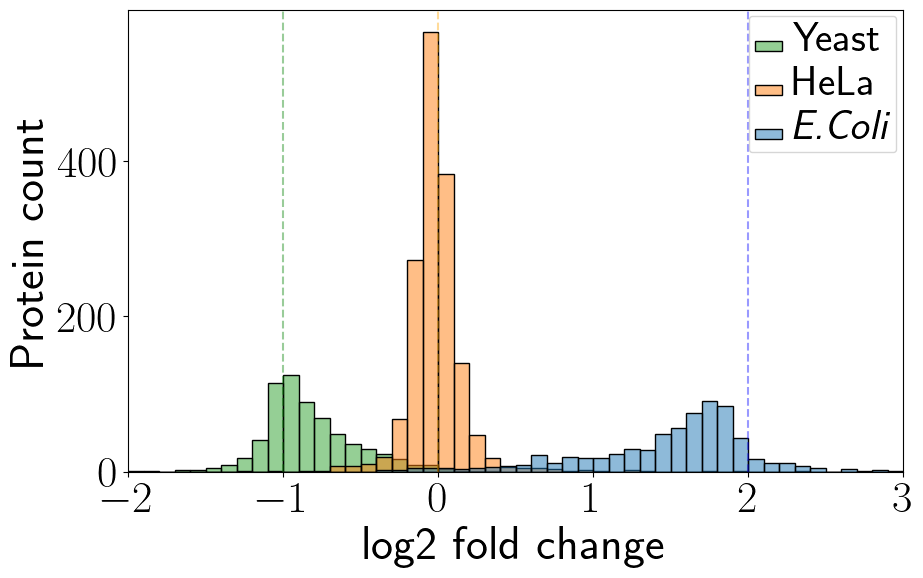
\includegraphics[width=0.4\linewidth]{../../result/report_plots_pipeline/histogram_ID_triqler.png} & 
	    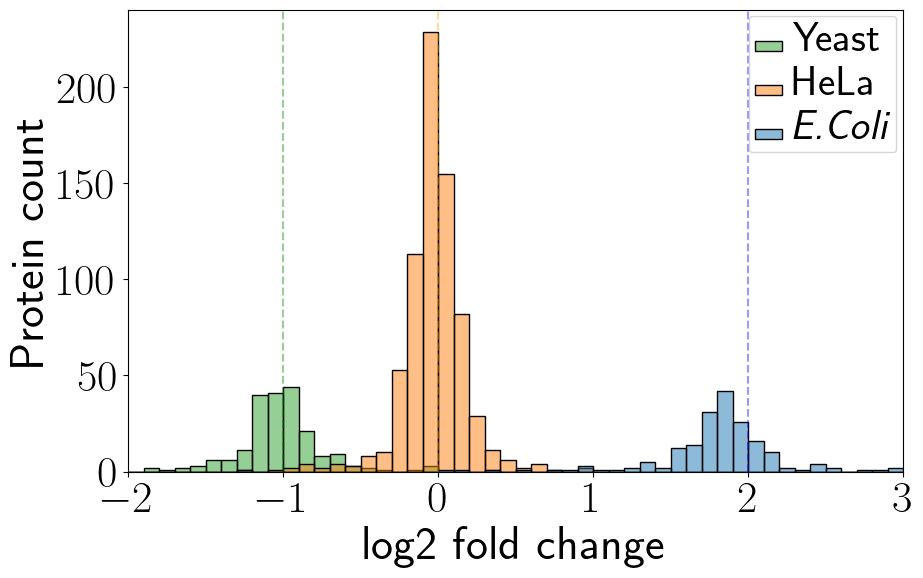
\includegraphics[width=0.4\linewidth]{../../result/report_plots_pipeline/histogram_ID_top3.png} \\ 
        A & B \\ 
	    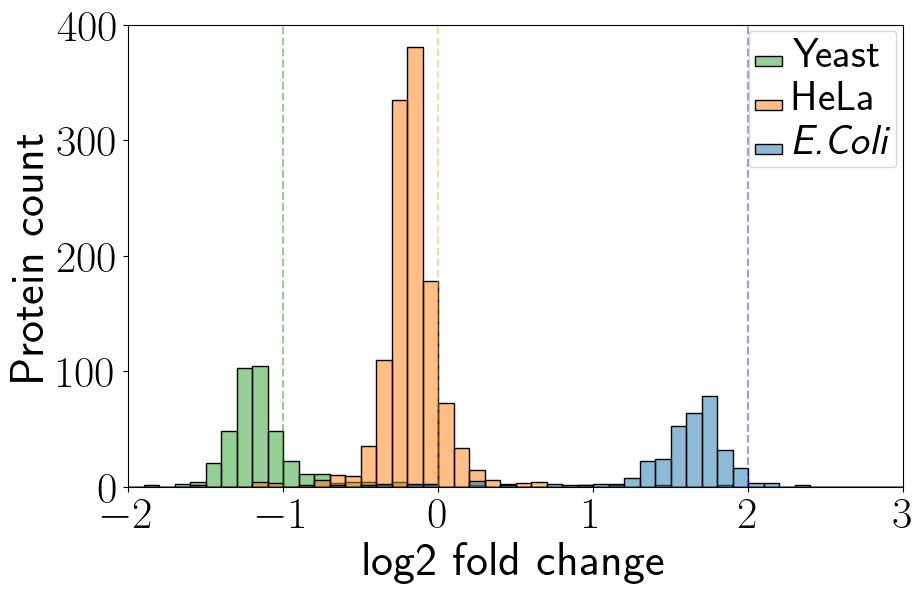
\includegraphics[width=0.4\linewidth]{../../result/report_plots_pipeline/histogram_ID_msstats.png} & 
	    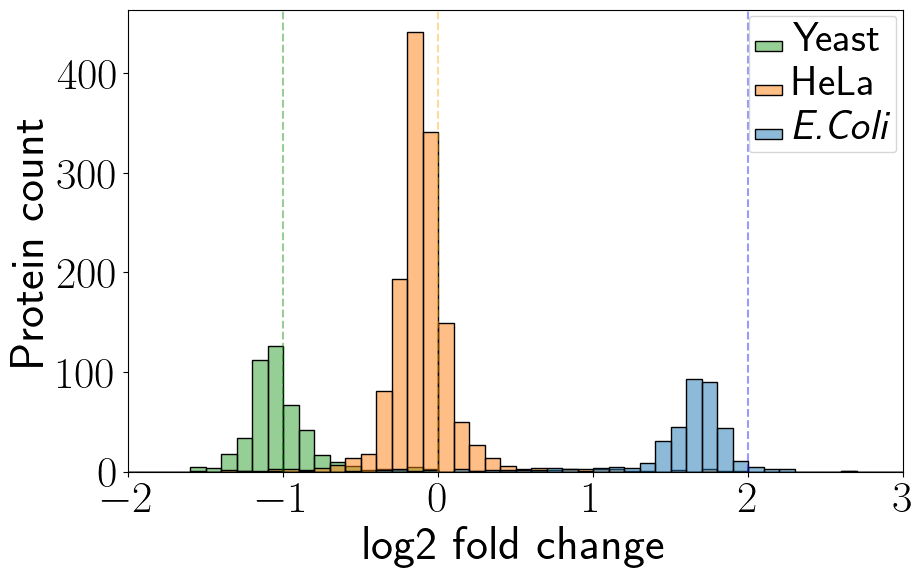
\includegraphics[width=0.4\linewidth]{../../result/report_plots_pipeline/histogram_ID_msqrob2.png} \\
        C & D 
    \end{tabular}
    \caption{{\bf Comparison of reported fold change distributions.} The summarized protein abundances from the ID spectral library pipeline for (A) Triqler, (B) Top3, (C) MSstats, and (D) MSqRob2 were binned and plotted as histograms. The dashed lines indicate the pipetted log2-fold change ratio between a specie and HeLa samples. We noted that the empirical densities of the protein counts are less biased for Triqler and Top3 than MSstats and MSqRob2, as the apex of their distribution was found closer to the true fold change difference (see Supplementary Figure \ref{fig:fc_histogram_supplement} for reported fold change distributions for both ID and PS workflows). For these histograms, we included all the summarized proteins and did not remove any proteins based on  the significance or fold change thresholds. \label{fig:fc_histogram}}
\end{figure}


\begin{figure}[hbt]
    \centering
    \begin{tabular}{ccc}
        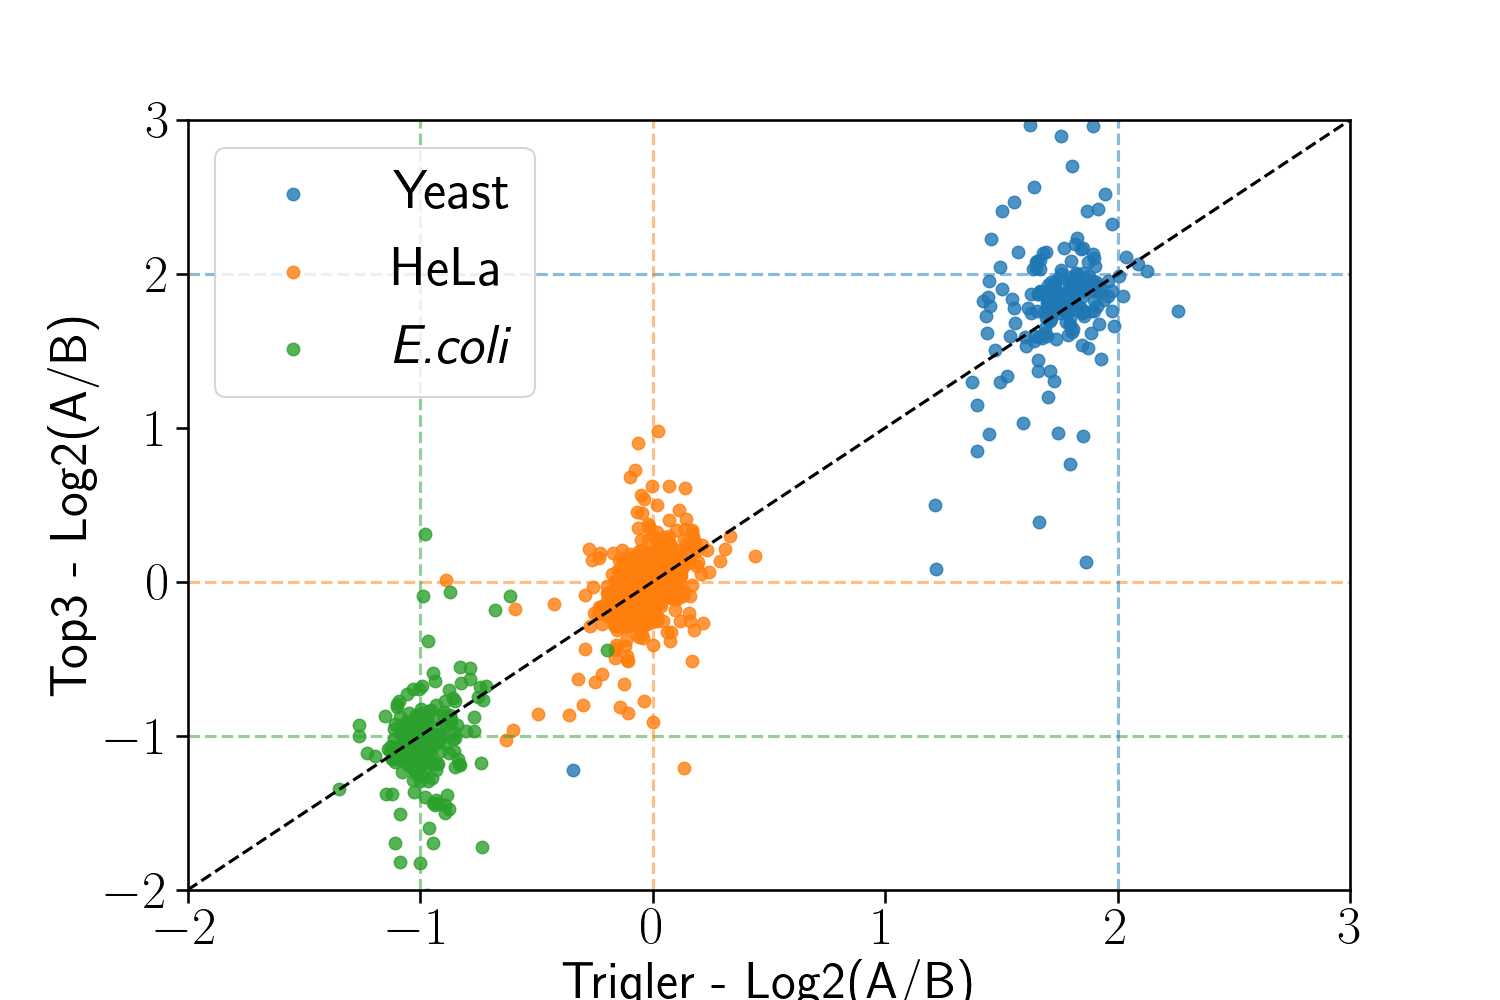
\includegraphics[width=0.33\linewidth]{../../result/report_plots_pipeline/scatter_ID_triqler_vs_top3.png} & 
        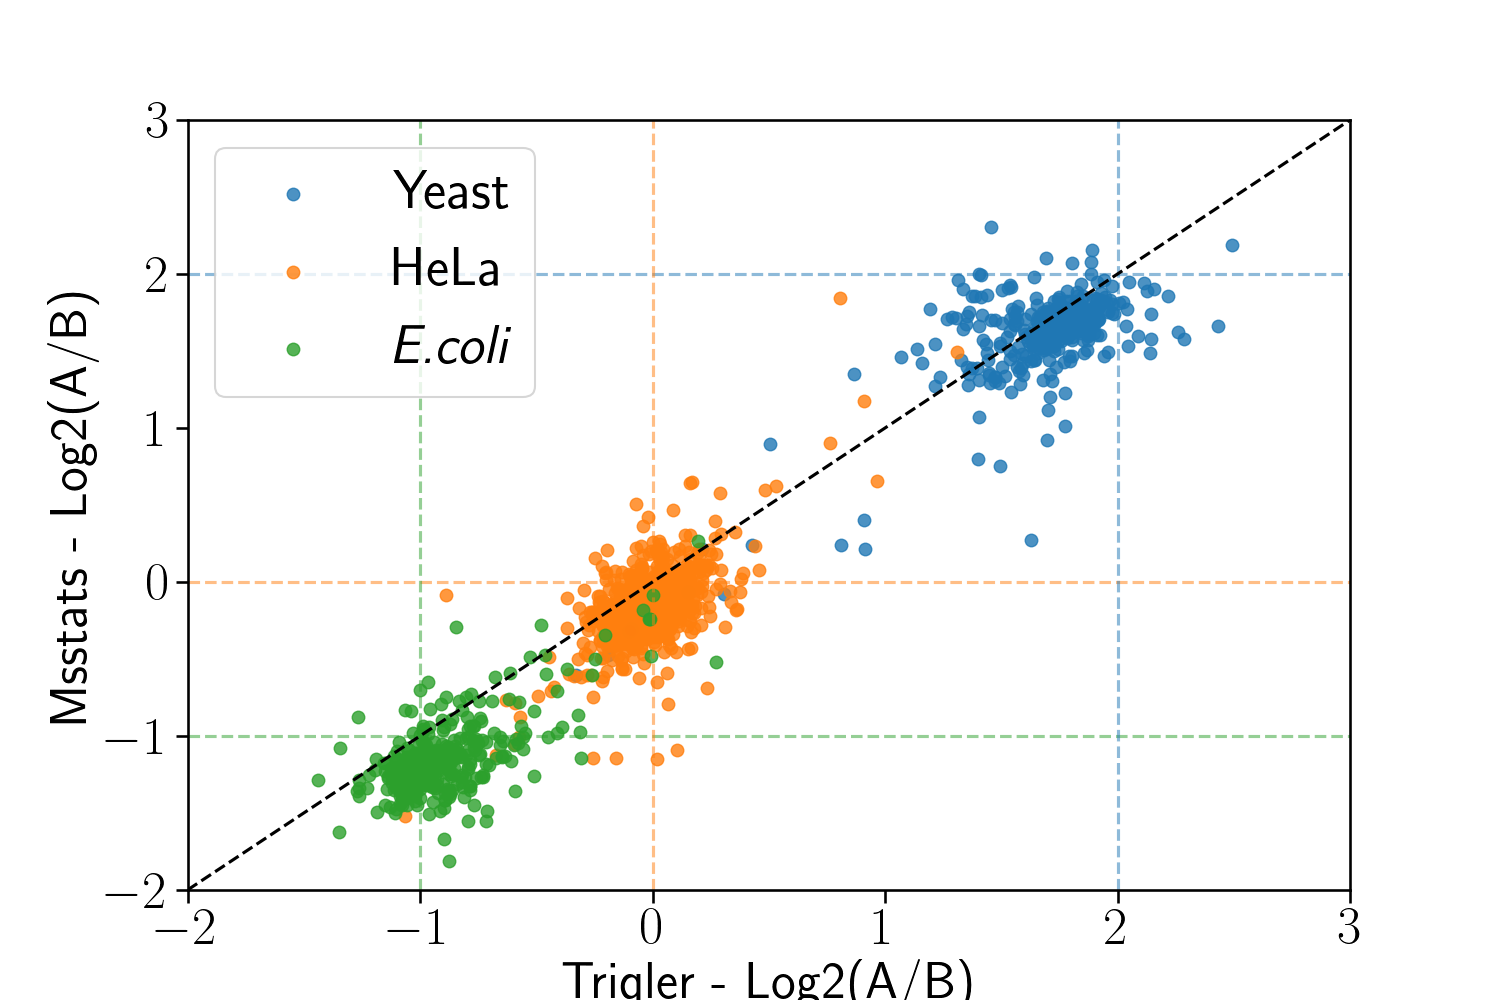
\includegraphics[width=0.33\linewidth]{../../result/report_plots_pipeline/scatter_ID_triqler_vs_msstats.png} & 
        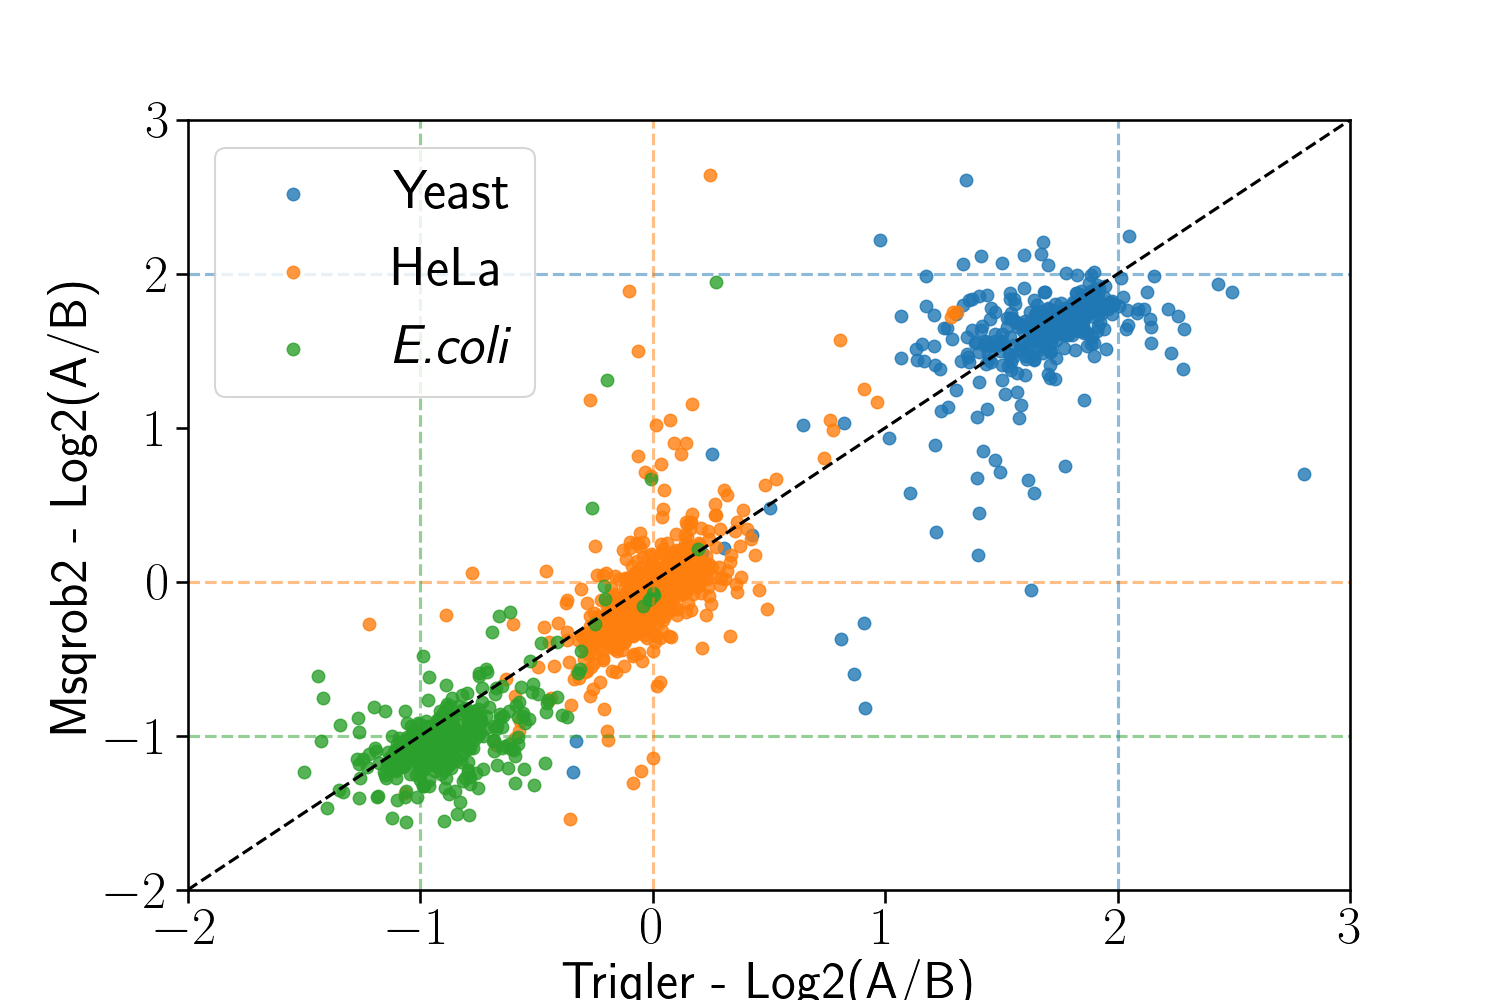
\includegraphics[width=0.33\linewidth]{../../result/report_plots_pipeline/scatter_ID_triqler_vs_msqrob2.png} \\
        A & B & C
    \end{tabular}
    \caption{{\bf Comparison of the summarized protein fold changes between the methods.} The comparison between the distributions of the MAP estimates from Triqler and (A) Top3, (B) MSstats, and (C) MSqRob2 for the data in the ID pipeline. The actual pipetted fold changes are indicated by dashed lines. Proteins not quantified by both compared methods were excluded from the plots. See Supplementary Figure \ref{fig:fc_scatter_supplement_triqler_vs_method_supplement} for protein-level results for both ID and PS workflows. \label{fig:fc_scatter}}
\end{figure}




\subsubsection*{Comparison of ability to discriminate differentially from equivalently abundant proteins}

As the first quantitative test of performance, we compared the methods' reported number of differentially abundant {\em E. Coli} and yeast proteins as a function of the number of HeLa proteins (Figure \ref{fig:diff_vs_hela}). As the former two lysates were injected in different concentrations and the HeLa was at constant concentration over the sample groups, a higher number of non-HeLa proteins for a similar number of HeLa-proteins is seen as better performance.  Overall, Triqler reports more such expected differentially abundant non-HeLa proteins per HeLa protein than the comparted methods for both the peptide abundances generated by the ID spectral library and PS spectral library pipelines. The results can be found in Supplementary Figure \ref{fig:ability_to_differentiate_differentially_abundant_specie_vs_hela}. To assure that our procedure to remove shared peptides before rather than after database matching, we also ran a second experiment where we removed shared peptides after matching. We found no large differances in removing peptides before or after database searching (Supplementary Figure \ref{fig:ability_to_differentiate_differentially_abundant_specie_vs_hela_full_lib}).

\begin{figure}[hbt]
    \centering
    \begin{tabular}{cc} 
        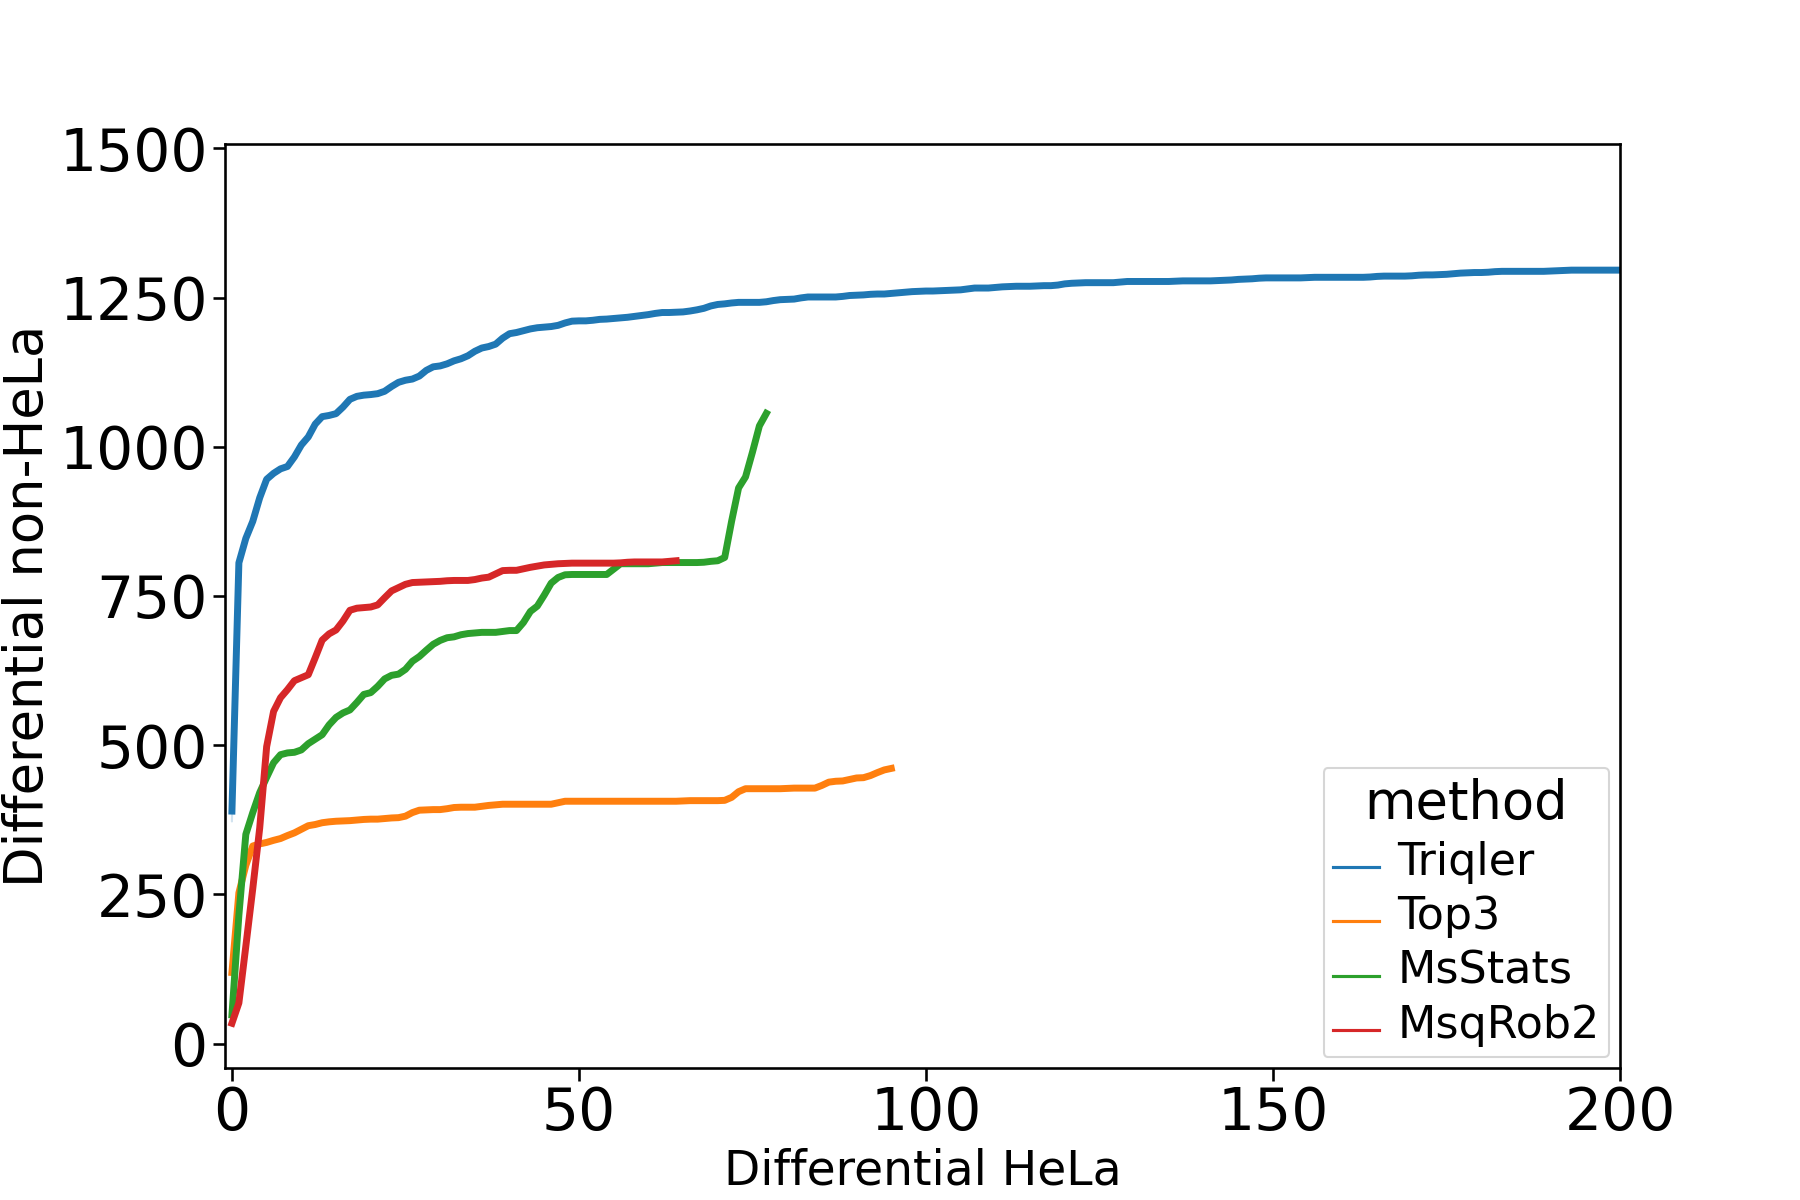
\includegraphics[width=0.45\linewidth]{../../result/report_plots_pipeline/diff_HeLa_vs_nonHeLa_ID_all_0.51.png} & 
        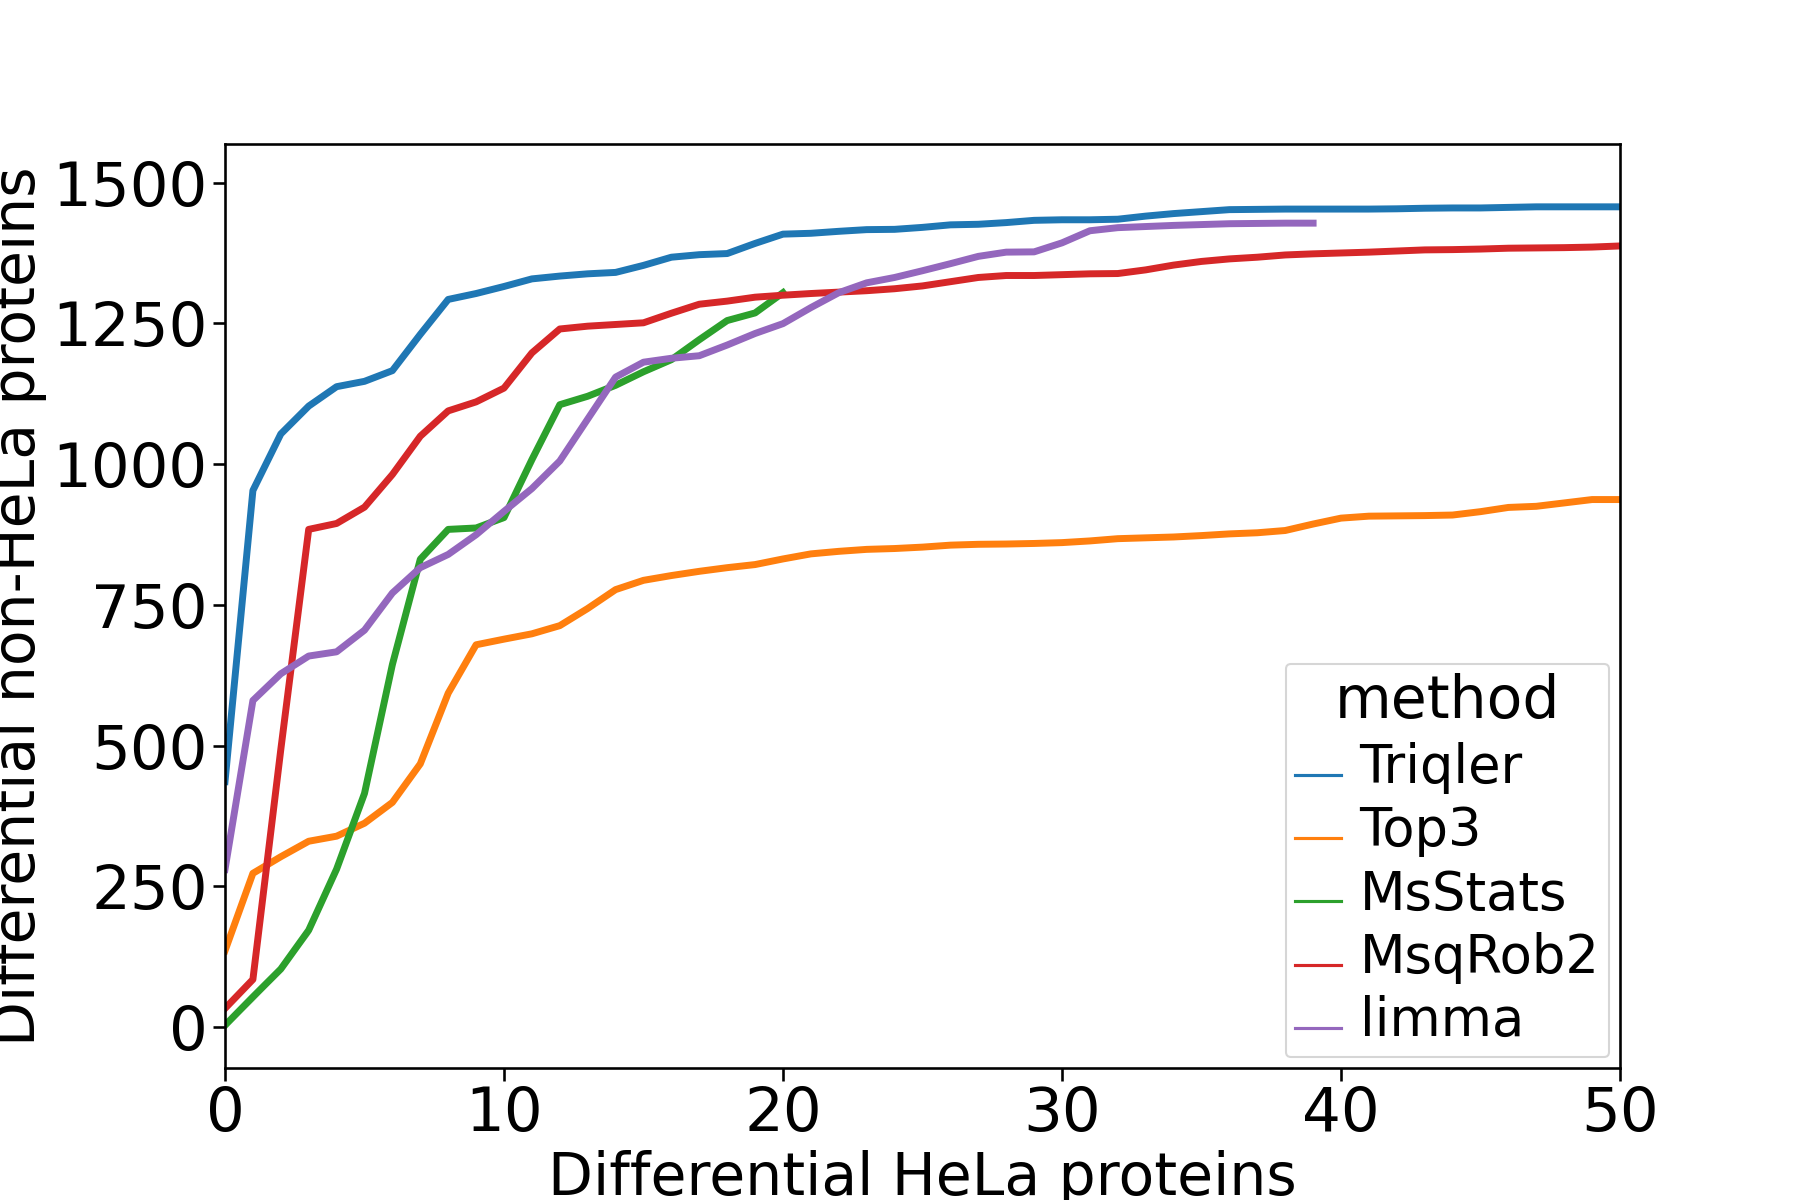
\includegraphics[width=0.45\linewidth]{../../result/report_plots_pipeline/diff_HeLa_vs_nonHeLa_PS_all_0.51_Limma.png}\\
        A & B 
    \end{tabular} 
    \caption{{\bf Comparison of ability to differentiate proteins with differential abundance between conditions.} We plotted the number of reported differentially abundant  {\em E. Coli} and yeast proteins as a function of the number of proteins from the HeLa background when sorting according to significance for (A) ID pipeline and (B) PS pipeline. For the test, we selected a fold change evaluation of 0.51 for Triqler and a fold change threshold of 0.51 for Top3, MSstats and MSqRob2. See the Supplement Figures \ref{fig:ability_to_differentiate_differentially_abundant_specie_vs_hela}-\ref{fig:ability_to_differentiate_differentially_abundant_specie_vs_hela_full_lib} for the number of differential abundant protein for each species. \label{fig:diff_vs_hela}}
\todo[inline]{Add a word 'protein' to the x/y labels. i.e. 'Differential HeLa proteins' and  'Differential non-HeLa proteins'}

\end{figure}

\subsubsection*{Comparison of statistical calibration}

Further, we tested the statistical calibration of the summarization methods. We hence investigated the relationship between the fraction of wrongly reported differential abundant proteins (i.e. the fraction of HeLa proteins among all reported differential abundant proteins), and each inference method's estimated false discovery rate (See Figure \ref{fig:frac_hela_vs_fdr} and Figure \ref{fig:frac_hela_vs_fdr_supp}). We observed that Triqler was better calibrated (closer to the diagonal line) than MSstats and MSqRob2. Top3 showed an even better calibration than Triqler but, as previously demonstrated, has a much lower sensitivity.

%We observed that Triqler, Top3, and MSqRob2 give estimates that are close to the true fold change level than MSstats. This is somewhat surprising given that both MSstats and MSqRob2 are using the Benjamini-Hochberger corrections which are generally found more conservative than $q$~value estimates.

%We observed that Triqler and Top3 were reporting slightly more accurate estimates than MSstats and MSqRobSum. This is somewhat surprising given that both MSstats and MSqRobSum are using the Benjamini-Hochberger corrections which are generally found more conservative than $q$~value estimates.

\begin{figure}[hbt]
    \centering
    \begin{tabular}{c} 
        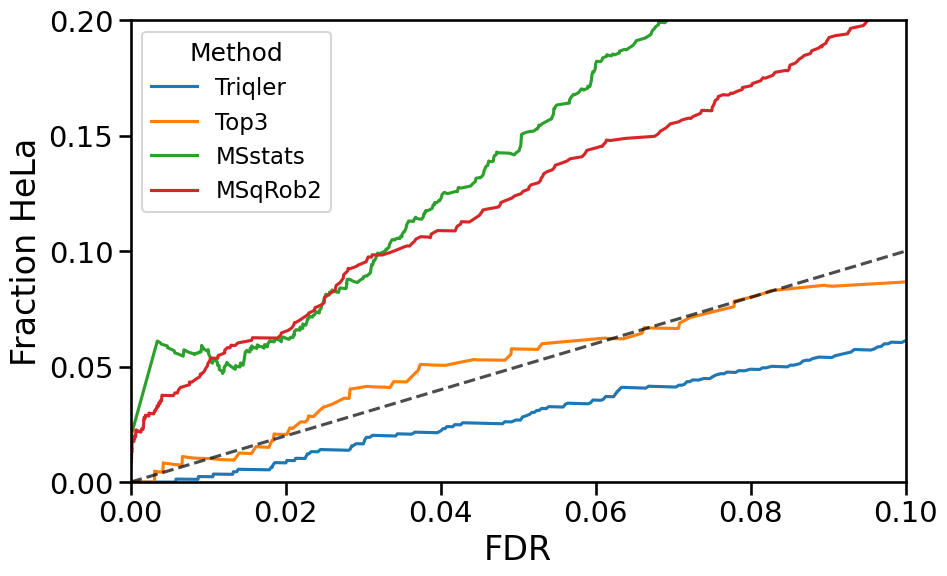
\includegraphics[width=0.5\linewidth]{../../result/report_plots_pipeline/calibration_ID_0.png}
    \end{tabular}
  \caption{{\bf Comparison of calibration of the compared summarization methods.} We plotted the fraction of reported differentially abundant HeLa proteins as a function of the $q$~value threshold for protein abundances without any restrictions on the fold change. We used $q$~value for Triqler and Top3, and Benjamini-Hochberg corrections for MSstats and MSqRob2. \label{fig:frac_hela_vs_fdr}}
\end{figure}

%\subsubsection*{Differential abundance reported by the protein quantification tools.}


%We also investigated the number of reported differential abundant proteins as reported by our four protein summarization methods. The results can be found in Supplementary Figure \ref{fig:ability_to_differentiate_differentially_abundant_specie_vs_hela}. Triqler reports the most differentially abundant proteins per .

\subsection*{Benchmark on non-engineered data}

To further compare the different protein inference methods, we finally tested their performance on a less engineered dataset, i.e. without known spiked concentrations of proteins. We hence downloaded data from Yang {\em et. al}~\cite{YANG2022104682}, a study of dorsal root ganglion (DRG) tissues of mice either injected or not injected with a cancer drug, Oxaliplatin, which is known to be neurotoxic in high concentrations. We processing the data through our PS pipeline followed by our protein summarization strategies, and plotted the number of differentially abundant proteins as a function of each methods estimated quantitative protein-level FDR of $q$~value (Figure~\ref{fig:non-engineered}). As can be seen from the data, Triqler outperforms the other methods, despite the fact that it, as previously shown, likely makes more conservative error estimates than the other methods.


\begin{figure}[hbt]
    \centering
    \begin{tabular}{c} 
        %\includegraphics[width=0.5\linewidth]{fixme} 
    \end{tabular}
  \caption{{\bf Reported performance of the compared methods on a non-engineered dataset.} We plotted the reported differentially abundant proteins as a function of their reported FDR/$q$~value without any restrictions on the fold change. \label{fig:non-engineered}}
  \todo[inline]{Figure here!}
\end{figure}


\section*{Discussion}

Here we have shown that Triqler operates well for DIA data, despite originally intended for DDA data. We also find that Triqler outperforms other protein summarization methods on an engineered benchmark set, both in terms of sensitivity and accuracy in its error estimates. Triqler was also able to detect a higher number of differentially abundant proteins at a more accurately reported false discovery rate than the compared methods. The absence of filtering and imputation steps before Triqler benefits the analysis by making it both more user-friendly by reducing parameter choices and inducing less bias into the result. 

The analytes in shotgun proteomics are peptides and not proteins or proteoforms. Nevertheless, most users of mass spectrometry use and will continue to find reasons to report findings on a protein level. It makes sense to put efforts into a better understanding of which protein inference tools to use at what occasion and how to summarize peptide abundances into protein relative concentration values. Also, protein summarization gives lower variance than peptide-level analysis, and it reduces the number of hypotheses tested and reduced the number of missing values, which can have a major impact on the quality of the analysis \cite{plubell2021can}.   

One important remark is that the sequence database that we used for matching the spectra was filtered so that only one protein per peptide was kept, to control for any difference in protein inference strategies used by our compared protein summarization methods. There is currently no consensus on how to handle multiple proteoforms in bottom-up proteomics. Hence, we believe that protein inference strategies that can account for multiple proteoforms would greatly benefit the field by improving the quality of the quantitative analysis. 

We also see some differences in how DIA and DDA peptide-level abundance data appear. For instance, there are more missing values in the DDA than in the DIA data. We addressed this issue by providing an alternative method for estimating the censoring function for missing values in Triqler.

It is quite hard to evaluate how the performance of a data processing pipeline is influenced by its components. This should not stop the field from trying to establish the features of the different processing steps \cite{dufresne2014abrf,gatto2016testing,navarro2016multicenter}. Unbiased comparisons of software tools are challenging for several reasons \cite{dufresne2014abrf}. Methods can be assessed by scientists lacking relevant expertise, the tested methods may be lacking sufficient documentation and the interpretation of test results may be subjective \cite{yates2012toward,leprevost2014best,pak2013clustering,faircomparison2015}. By using the same data set we can assure that the data set is processed consistently and further the analysis by extending it to protein summarization procedures.

Lastly, we want to highlight the benefit and importance of datasets such as the one provided by Navarro et al. \cite{navarro2016multicenter}. These benchmarking datasets make it easy for the scientific community to investigate computational tools by providing a golden standard and significantly facilitating benchmark studies. 

\section*{Funding}

This work was supported by grants from the Swedish Research Council (grant 2017-04030).

\section*{Supporting information}

\bibliographystyle{unsrt}
%\bibliography{benchmark}
\bibliography{benchmark.bib}
\end{document}



